%
% @author Kalvin Döge
%


\section{Stand der Wissenschaft}\label{sec:state-of-science}

Die Idee, Lichtsignalanlagen an Kreuzungen mit einer vorherbestimmten Steuerung zu verwalten, ist aber nicht keine neue.
Mehrere Forscher haben bereits Lösungen über künstliche Intelligenzen, durch Fokussierung auf die Fahrradfahrer oder zeitlicher Abstimmung von den Lichtsignalphasen gefunden.

\textbf{Li Kuang, Jianbo Zheng, Kemu Li und Honghao Gao:}
\textit{Intelligent Traffic Signal Control Based on Reinforcement Learning with State Reduction for Smart Cities}

In dem Forschungsbeitrag von Li Kuang und andere aus dem Jahr 2021, widmen sich die vier Autoren auf eine Lösung mithilfe eines Q-Learning-Algorithmus.
Dadurch, dass die Infrastruktur der Straßen nicht weiter ausgebaut werden kann in urbanem Verkehr, bleibt nur noch das Auflösen von Staus bei Lichtsignalschaltung und Kreuzungen\cite[S. 2]{Kuang2021}, weshalb sie sich mit dieser Arbeit an den Ansatz mit einer künstlichen Intelligenz setzten.

Die Aufgabe von bis entwickelten Echtzeitlösungsansätzen, so Kuang und andere, sind vier Kategorien zuzuordnen:
Feste Zeitschaltungen mit Anpassungen je Tageszeit, vorhersagende Signalschaltung aufgrund von Eingabedaten aus vergangenem oder aktuellem Verkehrsfluss, Betätigungssignalschaltung mit der bei Aktivierung von Sensoren Grün- oder Rotphasen verlängert werden und die Adaptivschaltung, die mit Sensoren und mit Algorithmen den Verkehr zum Zeitpunkt des Eintretens die Schaltungen verändern\cite[S. 2]{Kuang2021}.

Ihr Ansatz mit der künstlichen Intelligenz fällt unter eine neue Lösungsstrategie, mit der sie Lichtsignalphasen bei einzelnen Kreuzungen über das verstärkte Lernen abstimmen wollen\cite[S. 3]{Kuang2021}.
Beispielsweise sind gegenüberliegende, geradlinig gerichtete Straßenspuren, wie in der Grafik~\ref{fig:kuang-lanes} bei zum Beispiel den Spuren 6 und 2 zu sehen ist, miteinander verknüpfbar als eine Lichtsignalphase, da sie keine Überkreuzung ihrer Fahrbahn haben.
Um diese Phaseneinteilung für die künstliche Intelligenz vorzubereiten, sollen die einzelnen Fahrbahnen in Kombination mit Fahrzeugdaten in Gruppen unterteilt werden\cite[S. 6]{Kuang2021}.

\begin{figure}[h]
    \centering
    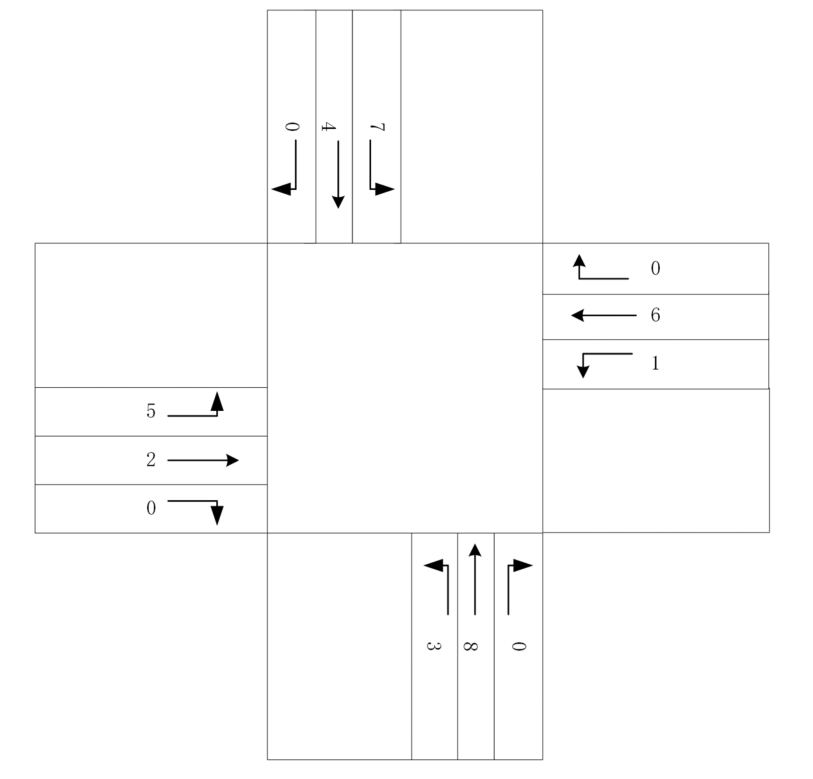
\includegraphics[width=0.75\textwidth]{kuang-lanes}~\caption{Das von Kuang und andere bei einer 3-spurigen Kreuzung dargelegte 8-Phasen Modell~\cite[S. 6]{Kuang2021}}
    \label{fig:kuang-lanes}
\end{figure}

Damit ließe sich der Algorithmus dann noch weiter verfeinern, als dass sie seltene oder fast nie auftretende Szenarien aus der Menge möglicher Zustände entfernen und sich nur die einzelnen Zahlen als Eingabe erhalten muss, nicht die gesamte Struktur der Kreuzung.

Im Folgenden gehen sie auf weitere Arbeiten ein, die eine andere Größenskalierungen als sie vorgenommen haben, bevor sie dann auf die genaue Implementation des Straßenmodells und dem Lernen beziehungsweise Trainieren der künstlichen Intelligenz eingehen.

Ein Problem bei der Phaseneinteilung ist aber, dass sie bei einzelnen Kreuzungen annahmen, dass jede Kreuzung je 3 eingehende Straßen hat, die in die Kreuzung münden.
Auch wenn die Stauzonen meist große Kreuzungen sind, so haben Städte auch Lichtsignalschaltungen verschiedene Kreuzungen mit mehr als nur 3 oder teilweise auch nur 2 Spuren, sodass ein Q-Learning-Algorithmus nicht mit solchen Szenarien umgehen kann und bei anderen Kreuzungen von vorne konzipiert und trainiert werden muss.

Dennoch ist die Einteilung der verschiedenen Lösungsansätze ein wichtiger Aspekt, der auch in dieser Arbeit Relevanz hat, explizit der erste Typ, die feststehende Zeitschaltung.


\textbf{Valentina Kurtc und Martin Treiber:}
\textit{Simulating bicycle traffic by the intelligent-driver model-Reproducing the traffic-wave characteristics observed in a bicycle-following experiment}

Der Forschungsbeitrag von Kurtc und Treiber aus dem Jahr 2020 untersucht die Hypothese, dass sich die Bewegungsdynamik des Fahrzeugverkehrs qualitativ nicht unterscheidet von dem Fahrradverkehr, indem sie die Qualität eines Fahrzeugmodells beziehungsweise Pkw-Modells ebenso für Fahrräder nutzen können.
Dies beweisen sie mit einem ,,Intelligent Driver Model``\cite[S. 20]{Kurtc2020}, einem mikroskopischen Modell für Autos, und vergleichen dessen Qualität der Kalibrierung und Vorhersagefähigkeit dann mit dem ,,Necessary Decelaration Model``\cite[S. 20]{Kurtc2020}, einem mikroskopischen Fahrradmodell.

Im Folgenden gehen Kurtc und andere darauf ein, wie sie eine Vergleichsbasis über die Formel herstellen und das anhand der Beschleunigungsfunktionen aus den Modellen aufbauen, um dann ein Kreisverkehrsszenario mit einem Fahrraddatenset zu simulieren und die berechneten Ergebnisse zu vergleichen.

\begin{figure}[h]
    \centering
    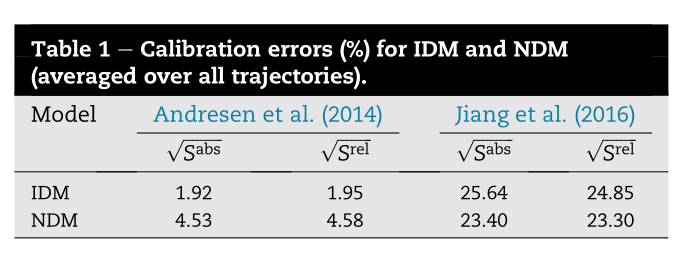
\includegraphics[width=0.75\textwidth]{kurtc2020}~\caption{die von Kurtc und Treiber berechneten, durchschnittlichen Kalbirierungsfehler der beiden Modelle in \%~\cite[S. 24]{Kurtc2020}}
    \label{fig:kurtc2020}
\end{figure}

Das Ergebnis aus der Grafik~\ref{fig:kurtc2020} zeigt, dass die Unterschiede der Modelle beim Nutzen von Fahrraddaten klein sind, als dass sie keinen großen Effekt auf die Simulationen haben.

Aus Kurtc und Treibers Forschungsarbeit lässt sich für diese Simulation also ableiten, dass Agenten, die auf der Straße fahren und Modalitäten wechseln, sowohl mit den Bewegungsmodellen von Fahrrad und Auto simuliert werden können, ohne an Akkuratheit einbüßen zu müssen.


\textbf{Saif Islam Bouderba und Najem Moussa:}
\textit{Reinforcement Learning (Q-LEARNING) traffic light controller within intersection traffic system}

In dem Thesenpapier von Bouderba und Moussa aus dem Jahr 2020 wird eine ähnliche Hypothese wie die von Kuang und andere untersucht.
Sie untersuchen die Effektivität von drei Lösungsansätzen für ihr zelluläres Automatenmodell sind:
Bei dem ersten Experiment simulieren sie einen einfachen, synchronisierten Ablauf der Lichtsignalschaltungen, beim Zweiten einen Ansatz einer ,,Grünen Welle``-Schaltung mit aufeinanderfolgenden Ampeln und beim Dritten eine durch Q-Learning-Algorithmus gesteuerte Kreuzungen~\cite[S. 2]{Bouderba2019}.

Ihr Automatenmodel besteht dabei aus einer Matrix an Kreuzungen, die alle von der Position her mit ihren umliegenden Nachbarn über eine zweispurige Straße verbunden sind:

\[N \times N = 4\]

Jede Kreuzung hat also vier Eingangs- und Ausgangspunkte sowie eine Lichtsignalanlage, die mit je einer Lösungsstrategie pro Experiment gesteuert wird.
Zudem ist die Simulationsumgebung aufgeteilt in Zellen, auf denen sich die Agenten entlangbewegen und zu den Kreuzungen gelangen\cite[S. 2]{Bouderba2019}.

\begin{figure}[h]
    \centering
    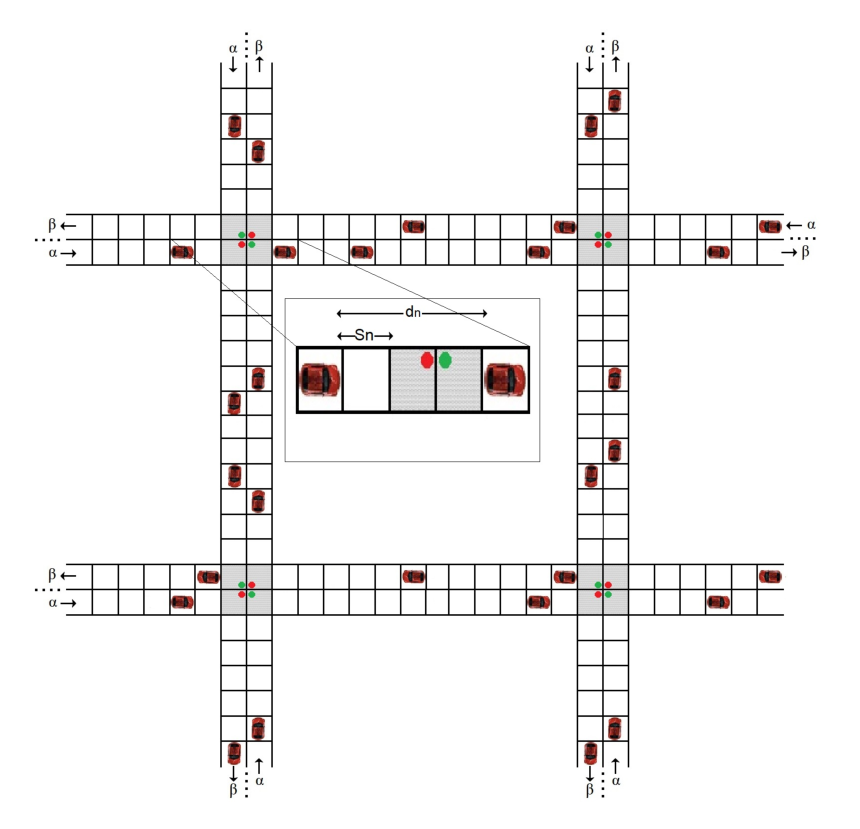
\includegraphics[width=0.75\textwidth]{bouderba-cells-model}~\caption{Eine Momentaufnahme aus dem zellulären Automatenmodell~\cite[S. 3]{Bouderba2019}}
    \label{fig:bouderba-cells-model}
\end{figure}

Mit dem Modell~\ref{fig:bouderba-cells-model} als Simulationsgrundlage erläutern Bouderba und Moussa die Lösungsstrategien.
Die grüne Welle Synchronisation erfolgt über eine Verschiebung der aktuellen, internen Zeituhr von umliegenden Lichtsignalen, während der Q-Learning-Alhorithmus trainiert wird, um eine passende Schaltung selbst zu erlernen.

\begin{figure}[h]
    \centering
    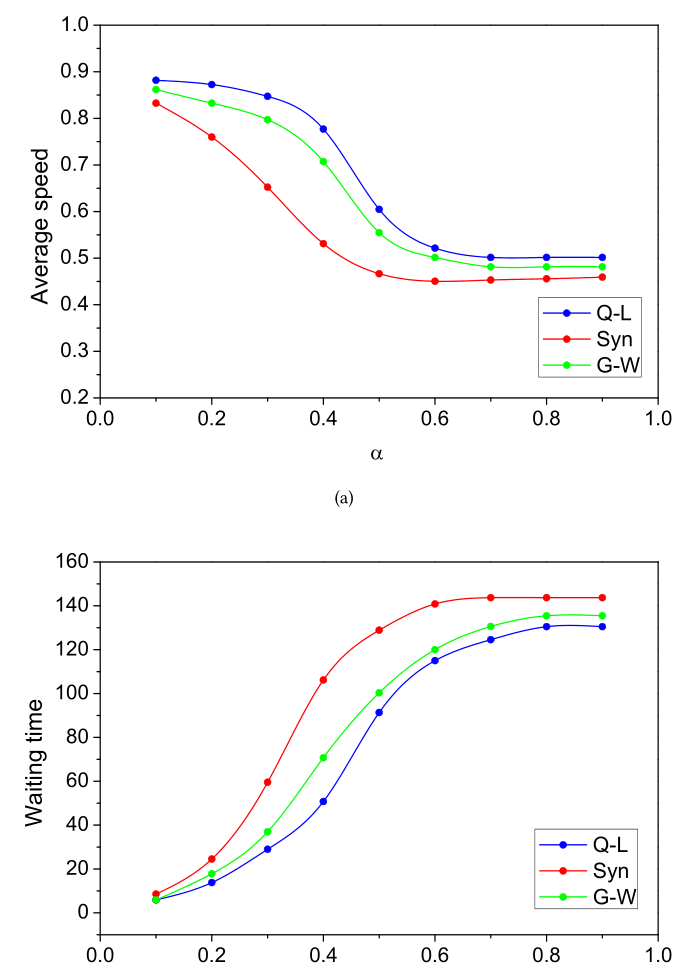
\includegraphics[width=0.5\textwidth]{bouderba-results}~\caption{Die durchschnittliche Geschwindigkeit und Wartezeit nach Durchführunge~\cite[S. 5]{Bouderba2019}}
    \label{fig:bouderba-result-graph}
\end{figure}


Die Resultate in Geschwindigkeit und Wartezeit pro Eingriffsrate aus Grafik~\ref{fig:bouderba-result-graph} zeigen auf, dass der einfache, synchronisierte Ansatz am schlechtesten von allen drei Algorithmen abschneidet.
Die durchschnittliche Wartezeit ist höher als die von dem Q-Learning-Algorithmus und der grünen Welle, genauso wie die durchschnittlichen Geschwindigkeitsmessungen niedriger ausfällt als bei den anderen beiden Ansätzen.

Auch wenn die Grüne-Welle-Schaltung in den Experimenten besser abschnitt, so ist dieser Ansatz nicht der dieser Arbeit.
Der Unterschied besteht darin, dass in Bouderba und Moussas Forschungsarbeit die Ampelphasenlängen auf ihrer Distanz basierend verlängert wurden.
Dies soll in dieser Arbeit aber durch eine insgesamt geltende Phasenschaltung ersetzt werden, da Agenten hier mehr als nur Geschwindigkeit erhöhen und senken können.
Sie können zum Beispiel kleine Veränderungen an Routen unternehmen, sodass sie nicht auf der Straße, sondern auf Fahrradwegen vorbeifahren und Lichtsignalschaltungen ignorieren.
Diese Bewegungsfreiheit der Agenten ist in dem Modell von Bouderba und Moussa nicht gegeben, weshalb die Forschungsarbeit nur als Motivation für die Verbesserungsmöglichkeiten einer grünen Welle angesehen werden kann.


\textbf{Katharina Mulack:}
\textit{Multiagenten Simulation von Fahrradfahrern im Kontext urbaner Verkehrsdynamik}

Die Masterarbeit von Katharina Mulack aus dem Jahr 2020 basiert ebenso auf dem MARS-Framework und ergänzt die bis zu dem Zeitpunkt der Arbeit in dem Framework fehlenden Fahrradfahrer.
Dabei fokussiert sich die Arbeit auf die detailreiche Rekonstruierung von Fahrradfahrern mit einem eigenen Bewegungsmodell, Statistiken über Eigenschaften von Fahrrädern und deren Interaktion mit der Umgebung\cite{Mulack2020}.
Bei den Verkehrsflussmodellen, einem Kernaspekt der Forschungsarbeit, wird insbesondere auf vier unterschiedliche Modellierungskonzepte eingegangen, die sich in der Feinheit der Simulationsmodelle unterscheiden:

Makroskopische Flussmodelle, die bei Simulationen sich mit dem allgemeinen Verlauf beschäftigen und die Details wie die Simulation einzelner Fahrzeuge nicht simulieren, um das Gesamtverhalten und ihr Effekt der Bewegung zu beobachten\cite[S. 6]{Mulack2020}.

Mikroskopische Modelle wiederum dienen der detaillierteren Simulation und beziehen individuelle Verhaltensweisen von Agenten mit der Umwelt oder anderen Agenten ein\cite[S. 6 f]{Mulack2020}.

Submikroskopische Modelle wiederum sind noch spezifischer und simulieren sogar Beziehungen zwischen Agenten und Entitäten, um den Detailgrad der echten Welt zu imitieren\cite[S. 7]{Mulack2020}.

Zuletzt wird noch das Mesoskopische Modell genannt, welches eine Mischung aus Makro- und Mikroskopmodell ist.
Bei diesem werden sowohl über große Distanzen und Gesamtverhalten angeschaut werden, dennoch aber die einzelnen Agenten oder Entitäten diese große Veranschaulichung ausmachen\cite[S. 7]{Mulack2020}.

Im Folgenden untersucht Mulacks Masterarbeit die Verkehrsflussmodelle und Statistiken über Fahrräder und implementiert sie zusammen mit neuen Umwelteinflüssen, den Lichtsignalanlagen.

Mulacks Forschungsarbeit selbst befasst sich mit einem hohen Detailgrad und zwischenagentlichen Beziehung bei den Fahrradfahrern, während sich diese Arbeit hier eher mit einem gemischten, mesoskopischen Simulationsmodell beschäftigt.
Zwar wird in dieser Arbeit ebenfalls auf einzelne Agenten benutzt, die mit ihrer Umwelt und den Entscheidungen andere Agenten beeinflussen, aber ist die generelle Stau- und Warteschlangenbildung wichtiger für die Ergebnisse.

Auch beschäftigt sich die Arbeit mehr mit dem Verhalten der Fahrradfahrer selbst innerhalb des MARS-Frameworks, nicht mit der Entwicklung einer optimalen Lichtsignalschaltung.
Dies macht diese Masterarbeit zu einer geeigneten Quelle für detailreiche Verhaltensweisen von Fahrrädern, weniger aber zu einem vergleichbaren Ansatz für diese Arbeit.
